\chapter{Infrastructure PKI et HashiCorp Vault}

\section{Conception de la hiérarchie de certification}

\subsection{Principes de conception}

L'infrastructure PKI adoptée suit une hiérarchie à \textbf{deux niveaux} : une CA racine et une CA intermédiaire. Ce schéma est recommandé par le NIST (SP 800-57) pour plusieurs raisons :

\begin{itemize}
  \item La CA racine peut rester hors-ligne (\textit{offline CA}), réduisant sa surface d'attaque.
  \item La CA intermédiaire, exposée aux systèmes applicatifs, peut être révoquée et remplacée sans invalider toute la chaîne.
  \item Les politiques de certification (contraintes de nommage, durées de vie) sont définies discriminément par niveau.
\end{itemize}

\begin{figure}[H]
  \centering
  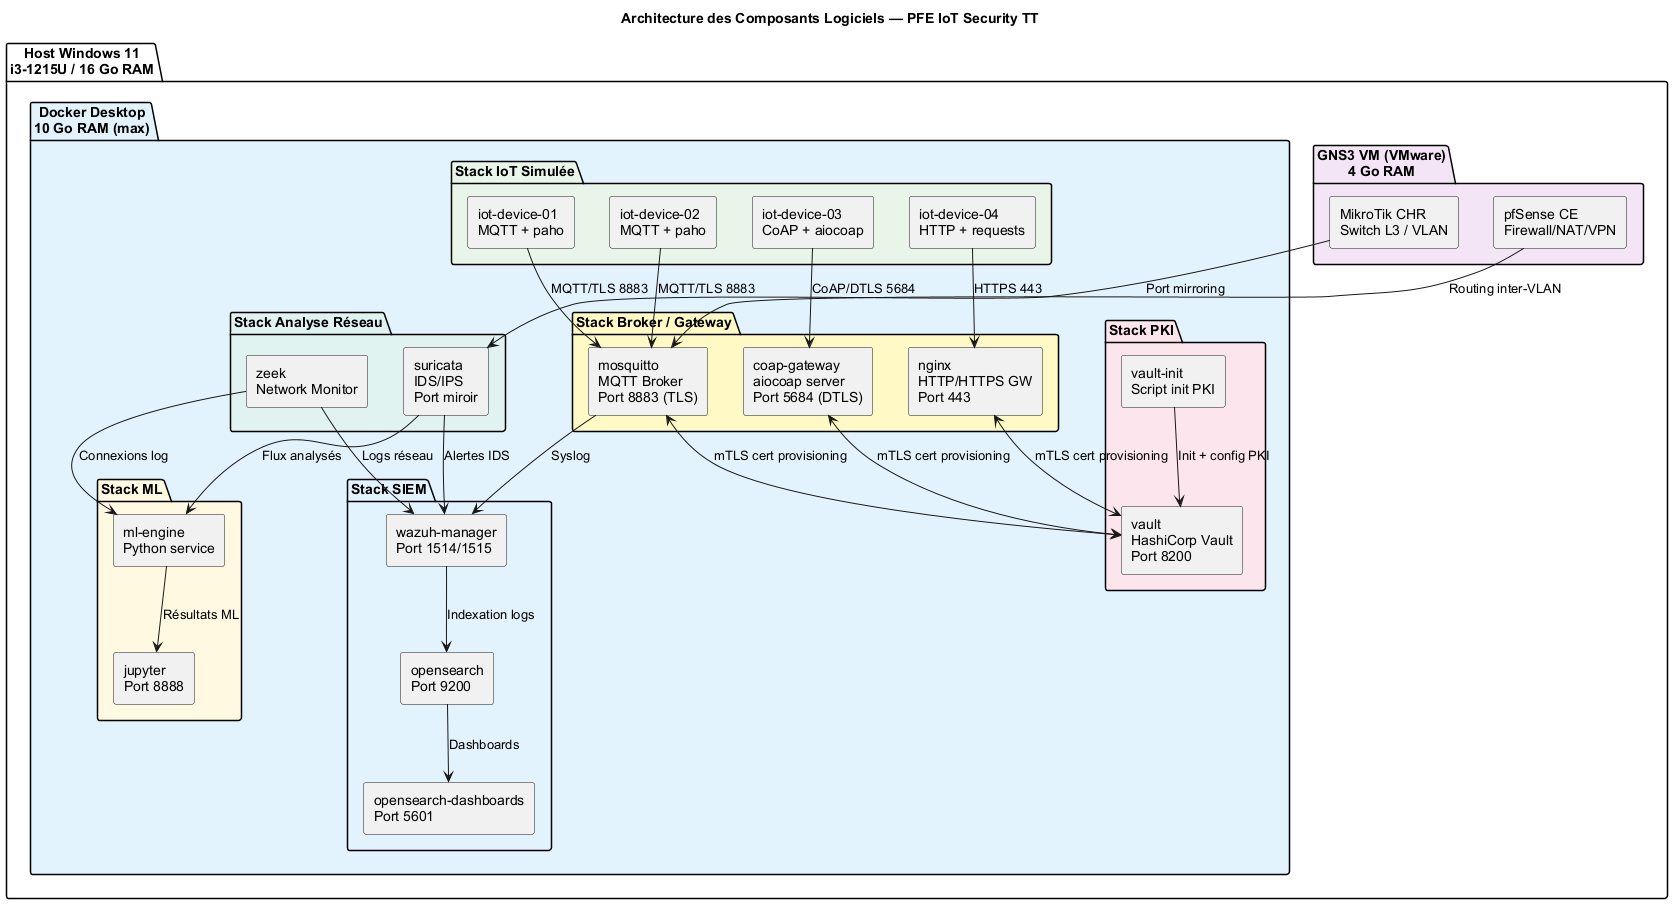
\includegraphics[width=0.7\textwidth]{figures/vault-pki-hierarchy.png}
  \caption{Hiérarchie PKI avec HashiCorp Vault}
  \label{fig:vault_pki}
\end{figure}

\subsection{Paramètres cryptographiques}

\begin{table}[H]
\centering
\caption{Paramètres cryptographiques de la PKI}
\label{tab:pki_params}
\begin{tabular}{lll}
\toprule
\textbf{Paramètre} & \textbf{CA Racine} & \textbf{CA Intermédiaire} \\
\midrule
Algorithme de clé & RSA-4096 & RSA-2048 \\
Algorithme de signature & SHA-256 & SHA-256 \\
Durée de validité & 10 ans & 5 ans \\
Profil de certificat & CA basic constraint & CA basic constraint \\
\bottomrule
\end{tabular}
\end{table}

Pour les certificats \textbf{dispositifs et services}, les paramètres sont :
\begin{itemize}
  \item \textbf{Algorithme} : RSA-2048 / SHA-256.
  \item \textbf{Validité} : 24 heures (dispositifs IoT — renouvellement automatique via script).
  \item \textbf{SAN (Subject Alternative Name)} : Inclut l'IP de la machine et le nom DNS.
  \item \textbf{Key Usage} : \texttt{digitalSignature, keyEncipherment}.
  \item \textbf{Extended Key Usage} : \texttt{clientAuth} (dispositifs), \texttt{serverAuth} (Mosquitto).
\end{itemize}

\section{Déploiement de HashiCorp Vault}

\subsection{Configuration initiale}

Vault est déployé dans un conteneur Docker basé sur l'image officielle \texttt{hashicorp/vault:1.15}. Il est configuré en mode \textbf{development} pour ce prototype, avec un backend de stockage en mémoire. Pour un déploiement production, un backend Consul ou Raft (intégré) serait recommandé.

\begin{lstlisting}[language=bash, caption=Initialisation de Vault et activation du moteur PKI]
# Initialisation et récupération des clés unseal
vault operator init -key-shares=3 -key-threshold=2

# Déverrouillage (unseal)
vault operator unseal <key-1>
vault operator unseal <key-2>

# Authentification avec le root token
vault login <root-token>

# Activation du moteur PKI racine
vault secrets enable -path=pki pki
vault secrets tune -max-lease-ttl=87600h pki
\end{lstlisting}

\subsection{Création de la CA racine}

\begin{lstlisting}[language=bash, caption=Génération de la CA racine dans Vault]
vault write -field=certificate pki/root/generate/internal \
    common_name="PFE-IoT Root CA" \
    issuer_name="root-2024" \
    ttl=87600h \
    key_type=rsa \
    key_bits=4096 > /pki/certs/ca/root-ca.crt
\end{lstlisting}

\subsection{Création de la CA intermédiaire}

\begin{lstlisting}[language=bash, caption=Génération et signature de la CA intermédiaire]
# Activation du moteur PKI intermédiaire
vault secrets enable -path=pki_int pki
vault secrets tune -max-lease-ttl=43800h pki_int

# Génération du CSR intermédiaire
vault write -format=json pki_int/intermediate/generate/internal \
    common_name="PFE-IoT Intermediate CA" | \
    jq -r '.data.csr' > /tmp/pki_int.csr

# Signature par la CA racine
vault write -format=json pki/root/sign-intermediate \
    issuer_ref="root-2024" \
    csr=@/tmp/pki_int.csr \
    format=pem_bundle \
    ttl=43800h | \
    jq -r '.data.certificate' > /tmp/pki_int.crt

# Import du certificat signé dans le moteur intermédiaire
vault write pki_int/intermediate/set-signed \
    certificate=@/tmp/pki_int.crt
\end{lstlisting}

\subsection{Définition des rôles d'émission}

Deux rôles sont définis pour contrôler les types de certificats émissibles :

\begin{lstlisting}[language=bash, caption=Rôles Vault pour services et dispositifs IoT]
# Rôle pour les services (Mosquitto, etc.)
vault write pki_int/roles/services \
    allowed_domains="pfe-iot.local" \
    allow_subdomains=true \
    allow_ip_sans=true \
    key_type=rsa key_bits=2048 \
    max_ttl=8760h

# Rôle pour les dispositifs IoT (durée courte)
vault write pki_int/roles/iot-devices \
    allowed_domains="devices.pfe-iot.local" \
    allow_subdomains=true \
    allow_ip_sans=true \
    key_type=rsa key_bits=2048 \
    max_ttl=24h
\end{lstlisting}

\section{Émission automatique des certificats de dispositifs}

Le script \texttt{generate\_device\_certs.sh} automatise l'émission d'un certificat par dispositif simulé :

\begin{lstlisting}[language=bash, caption=Émission d'un certificat de dispositif via l'API Vault]
#!/bin/bash
DEVICE_ID=$1
VAULT_ADDR="http://192.168.20.20:8200"
VAULT_TOKEN="${VAULT_TOKEN}"

# Appel API Vault pour émettre le certificat
curl -s -X POST \
  "${VAULT_ADDR}/v1/pki_int/issue/iot-devices" \
  -H "X-Vault-Token: ${VAULT_TOKEN}" \
  -d "{\"common_name\": \"${DEVICE_ID}.devices.pfe-iot.local\", \"ttl\": \"24h\"}" | \
  python3 -c "
import sys, json
data = json.load(sys.stdin)['data']
open(f'certs/{DEVICE_ID}.crt', 'w').write(data['certificate'])
open(f'certs/{DEVICE_ID}.key', 'w').write(data['private_key'])
open(f'certs/ca-chain.crt', 'w').write(data['ca_chain'][0])
"
\end{lstlisting}

\section{Validation de la PKI}

La chaîne de certification est validée avec \texttt{openssl verify} :

\begin{lstlisting}[language=bash, caption=Validation de la chaîne de certification]
# Vérification de la chaîne complète
openssl verify -CAfile pki/certs/ca/root-ca.crt \
               -untrusted pki/certs/ca/intermediate-ca.crt \
               pki/certs/devices/device-001.crt

# Résultat attendu :
# pki/certs/devices/device-001.crt: OK

# Inspection du certificat
openssl x509 -in pki/certs/devices/device-001.crt \
             -noout -text | grep -A5 "Subject:"
\end{lstlisting}

\begin{tcolorbox}[colback=green!5, colframe=green!50!black, title=Résultat PKI]
\textbf{50 certificats de dispositifs} émis avec succès via l'API Vault. Chaîne de confiance validée : dispositif $\to$ CA intermédiaire $\to$ CA racine. Durée d'émission moyenne : \textbf{87 ms} par certificat via API REST.
\end{tcolorbox}
